\documentclass[11pt,a4paper]{report}
\usepackage{amsmath}
\usepackage{amssymb}

\usepackage{graphicx}

\usepackage{listings}
\usepackage{color} %red, green, blue, yellow, cyan, magenta, black, white
\definecolor{mygreen}{RGB}{28,172,0} % color values Red, Green, Blue
\definecolor{mylilas}{RGB}{170,55,241}
\usepackage[utf8]{inputenc}
\usepackage[english]{babel}
\usepackage{booktabs}

\usepackage{graphicx}


\begin{document}
\section{Problem}
We are solving this problem:
\begin{gather*}
J(y,u) = \frac{1}{2}\int_0^Tu^2dt + \frac{1}{2}(y(T)-y^T)^2
\end{gather*} 
and let our ODE constraint be:
\begin{align*}
\left\{
     \begin{array}{lr}
       	E(y,u) = y'-\alpha y -u\\
       	   y(0)=y_0
     \end{array}
   \right.
\end{align*}
To do this we need the gradient of the reduced $J$, which is:
\begin{align*}
\nabla\hat{J} = u+p
\end{align*}
p is the solution of the adjoint equation:
\begin{align*}
   \left\{
     \begin{array}{lr}
       -p'(t) -\alpha p(t)=0  \\
       p(T) = y(T)-y^T
     \end{array}
   \right.
\end{align*}
Because we want to parallelize in time we also try to solve the control problem with added penalty terms:
\begin{align*}
J(y,u,\lambda) = \int_0^T u^2 dt + \frac{1}{2}(y_m(T)-y^T)^2 + \frac{\mu}{2} \sum_{i=1}^{m-1} (y_{i}(T_i)-\lambda_i)^2 
\end{align*}
This functional has the following gradient:
\begin{align*}
\hat{J}'(u,\lambda) = (u+p,p_{2}(T_1) -p_{1}(T_1),..., p_{m}(T_{m-1}) -p_{m}(T_{m-1}))
\end{align*} 
We now also solve the state equations:
\begin{align*}
   \left\{
     \begin{array}{lr}
       \frac{\partial }{\partial t} y_i(t) = \alpha y_i(t) + u(t) \ \text{for $t \in [T_{i-1},T_{i}]$}\\
	y_i(T_{i-1}) = \lambda_{i-1}
     \end{array}
   \right.
\end{align*}
and the adjoint equations:
\begin{align*}
-\frac{\partial }{\partial t}p_m &=\alpha p_m  \\
p_m(T_{m}) &= y_m(T_{m})-y_T
\end{align*}
On $[T_{i-1},T_i]$ the adjoint equation is:
\begin{align*}
-\frac{\partial }{\partial t}p_i &=p_i  \\
p_i(T_{i}) &= \mu(y_{i}(T_{i})-\lambda_{i} )
\end{align*}
\section{Assumption}
Assume that we have solved the non-penalty problem, and have an optimal control $u^*$ and a corresponding solution to the state equation $y^*$. What happens if we try to solve the same problem using the penalty method with $u*$ and $\lambda_i =y^*(T_i)$ as an initial guess? One might expect that $u*$ would also be optimal for the penalty method with any choise of $\mu$. This is however not the case, and we see why, by calculating the gradient using the initial guess. The problem is that the adjoint equation in all subintervals except the last have initial condition 0. This results what is shown in plot below. If we then solve the problem using $u^*$ as initial guess, we will eventually get a solution close to $u^*$, but it will not be exactly the same.
\\
\\
Even though $u^*$ is not a valid solution for the penalty method, using it as initial guess allows us to come arbitrary close to the real non-penalty solution if solve it using increasing $\mu$ values.
\\
\\ 
\begin{tabular}{lrr}
\toprule
{} &             $\mu$ &    $||u-u_{\mu}||_{L^2}$ \\
\midrule
0  &             10 &  3.298276e-01 \\
1  &            100 &  4.510803e-06 \\
2  &           1000 &  4.620845e-07 \\
3  &          10000 &  4.632146e-08 \\
4  &         100000 &  4.633279e-09 \\
5  &        1000000 &  4.633392e-10 \\
6  &       10000000 &  4.633403e-11 \\
7  &      100000000 &  4.633407e-12 \\
8  &     1000000000 &  4.633409e-13 \\
9  &    10000000000 &  4.632983e-14 \\
10 &   100000000000 &  4.689641e-15 \\
11 &  1000000000000 &  6.090340e-16 \\
\bottomrule
\end{tabular}
\\
\\
I solve the mentioned problem for different time-decompositions and time-steps  using the parameters: $(y_0,y_T,T,a)=(1,-10,1,1)$. This yielded the following relative errors between penalty and non-penalty control solutions:
\\
\\
$N=100$:
\\
\begin{tabular}{lrrrrrr}
\toprule
{} $\mu$&        2  &        4  &        8  &        16 &        32 &        64 \\
\midrule
1.000000e+01 &  0.062196 &  0.174324 &  0.337817 &  0.522134 &  0.692612 &  0.808695 \\
1.000000e+02 &  0.007483 &  0.020676 &  0.048616 &  0.098498 &  0.183879 &  0.297111 \\
1.000000e+03 &  0.001420 &  0.002115 &  0.005161 &  0.010805 &  0.022035 &  0.040562 \\
1.000000e+04 &  0.001411 &  0.000211 &  0.000634 &  0.001120 &  0.002248 &  0.004235 \\
1.000000e+05 &  0.001410 &  0.000170 &  0.000417 &  0.000653 &  0.001323 &  0.000404 \\
1.000000e+06 &  0.001410 &  0.000170 &  0.000416 &  0.000653 &  0.001298 &  0.000403 \\
1.000000e+07 &  0.001410 &  0.000170 &  0.000416 &  0.000651 &  0.001294 &  0.000402 \\
1.000000e+08 &  0.001410 &  0.000170 &  0.000416 &  0.000651 &  0.001294 &  0.000402 \\
1.000000e+09 &  0.001410 &  0.000170 &  0.000416 &  0.000651 &  0.001294 &  0.000402 \\
1.000000e+10 &  0.001410 &  0.000170 &  0.000416 &  0.000651 &  0.001294 &  0.000402 \\
1.000000e+13 &  0.001410 &  0.000170 &  0.000416 &  0.000651 &  0.001294 &  0.000402 \\
\bottomrule
\end{tabular}
\\
$N=1000$:
\\
\begin{tabular}{lrrrrrr}
\toprule
{} $\mu$&        2  &        4  &        8  &        16 &        32 &        64 \\
\midrule
1.000000e+01 &  0.061013 &  0.174237 &  0.338846 &  0.527739 &  0.699207 &  0.825213 \\
1.000000e+02 &  0.006545 &  0.020662 &  0.048753 &  0.100515 &  0.188610 &  0.320711 \\
1.000000e+03 &  0.000731 &  0.002105 &  0.005099 &  0.011051 &  0.022720 &  0.045084 \\
1.000000e+04 &  0.000127 &  0.000211 &  0.000513 &  0.001116 &  0.002322 &  0.004699 \\
1.000000e+05 &  0.000127 &  0.000021 &  0.000052 &  0.000112 &  0.000236 &  0.000472 \\
1.000000e+06 &  0.000127 &  0.000002 &  0.000006 &  0.000009 &  0.000025 &  0.000047 \\
1.000000e+07 &  0.000127 &  0.000002 &  0.000006 &  0.000009 &  0.000015 &  0.000002 \\
1.000000e+08 &  0.000127 &  0.000002 &  0.000006 &  0.000009 &  0.000015 &  0.000002 \\
1.000000e+09 &  0.000127 &  0.000002 &  0.000006 &  0.000009 &  0.000015 &  0.000002 \\
1.000000e+10 &  0.000127 &  0.000002 &  0.000006 &  0.000009 &  0.000015 &  0.000002 \\
1.000000e+13 &  0.000127 &  0.000002 &  0.000006 &  0.000009 &  0.000015 &  0.000002 \\
\bottomrule
\end{tabular}
\\
$N=10000$:
\\
\begin{tabular}{lrrrrrr}
\toprule
{} $\mu$&        2  &            4  &            8  &        16 &        32 &        64 \\
\midrule
1.000000e+01 &  0.060877 &  1.742088e-01 &  3.388225e-01 &  0.528336 &  0.700282 &  0.826652 \\
1.000000e+02 &  0.006450 &  2.066013e-02 &  4.874753e-02 &  0.100732 &  0.189396 &  0.322893 \\
1.000000e+03 &  0.000656 &  2.105155e-03 &  5.098720e-03 &  0.011077 &  0.022831 &  0.045517 \\
1.000000e+04 &  0.000071 &  2.109139e-04 &  5.124423e-04 &  0.001119 &  0.002331 &  0.004746 \\
1.000000e+05 &  0.000011 &  2.109436e-05 &  5.143613e-05 &  0.000112 &  0.000234 &  0.000477 \\
1.000000e+06 &  0.000011 &  2.108745e-06 &  7.348341e-06 &  0.000011 &  0.000023 &  0.000048 \\
1.000000e+07 &  0.000011 &  1.416372e-07 &  7.348085e-06 &  0.000011 &  0.000002 &  0.000048 \\
1.000000e+08 &  0.000011 &  6.703425e-08 &  6.248438e-07 &  0.000011 &  0.000002 &  0.000048 \\
1.000000e+09 &  0.000011 &  6.702827e-08 &  6.248447e-07 &  0.000011 &  0.000002 &  0.000048 \\
1.000000e+10 &  0.000011 &  6.702827e-08 &  6.248447e-07 &  0.000011 &  0.000002 &  0.000048 \\
1.000000e+13 &  0.000011 &  6.702823e-08 &  6.248448e-07 &  0.000011 &  0.000002 &  0.000048 \\
\bottomrule
\end{tabular}
\\
Now for the same problem with slightly different parameters: $(y_0,y_T,T,a)=(3.3,10,1,1.4)$, I used a constant number of time-decompositions, while decreasing the time-steps. Here are some results:
\\
$m=2$:
\\
\begin{tabular}{lrrrrrrrr}
\toprule
{} &     101   &     501   &         801   &         1001  &         2000  &         5000  &         10000 &         50000 \\
\midrule
1e+00 &  0.386457 &  0.384180 &  3.839e-01 &  3.838e-01 &  3.835e-01 &  3.836e-01 &  3.836e-01 &  3.836e-01 \\
1e+01 &  0.059256 &  0.058724 &  5.867e-02 &  5.865e-02 &  5.858e-02 &  5.858e-02 &  5.858e-02 &  5.858e-02 \\
1e+02 &  0.006260 &  0.006200 &  6.194e-03 &  6.192e-03 &  6.184e-03 &  6.184e-03 &  6.184e-03 &  6.184e-03 \\
1e+04 &  0.000063 &  0.000062 &  6.233e-05 &  6.230e-05 &  6.223e-05 &  6.210e-05 &  6.202e-05 &  6.193e-05 \\
1e+05 &  0.000058 &  0.000006 &  6.398e-06 &  6.263e-06 &  6.223e-06 &  6.170e-06 &  6.020e-06 &  5.967e-06 \\
1e+06 &  0.000058 &  0.000005 &  5.765e-07 &  7.675e-07 &  6.225e-07 &  5.632e-07 &  5.995e-07 &  7.416e-07 \\
1e+07 &  0.000058 &  0.000005 &  5.754e-07 &  6.808e-07 &  6.221e-07 &  9.919e-08 &  5.995e-07 &  7.416e-07 \\
1e+08 &  0.000058 &  0.000005 &  5.753e-07 &  6.807e-07 &  6.220e-07 &  9.921e-08 &  5.995e-07 &  7.416e-07 \\
1e+09 &  0.000058 &  0.000005 &  5.753e-07 &  6.807e-07 &  6.220e-07 &  1.336e-07 &  5.995e-07 &  7.416e-07 \\
1e+10 &  0.000058 &  0.000005 &  5.753e-07 &  6.807e-07 &  6.220e-07 &  1.336e-07 &  5.995e-07 &  7.416e-07 \\
1e+13 &  0.000058 &  0.000005 &  5.753e-07 &  6.807e-07 &  6.220e-07 &  1.335e-07 &  5.995e-07 &  7.416e-07 \\
\bottomrule
\end{tabular}
\\
$m=7$:
\\
\begin{tabular}{lrr}
\toprule
{} &     100   &     50000 \\
\midrule
1.000000e+05 &  0.840806 &  0.000049 \\
1.000000e+06 &  0.836320 &  0.000049 \\
1.000000e+07 &  0.834409 &  0.000014 \\
1.000000e+08 &  0.834409 &  0.000014 \\
1.000000e+09 &  0.834405 &  0.000014 \\
2.000000e+09 &  0.834405 &  0.000014 \\
5.000000e+09 &  0.834404 &  0.000014 \\
1.000000e+10 &  0.834404 &  0.000014 \\
1.000000e+11 &  0.834404 &  0.000014 \\
\bottomrule
\end{tabular}
\\
$m=10$:
\\
\begin{tabular}{lrrrrrrrr}
\toprule
{} &     101   &     501   &     801   &     1001  &     2000  &     5000  &     10000 &     50000 \\
\midrule
1.000000e+00 &  0.876719 &  0.877567 &  0.877646 &  0.877675 &  0.877786 &  0.877784 &  0.877781 &  0.877776 \\
1.000000e+01 &  0.415605 &  0.417511 &  0.417692 &  0.417753 &  0.418012 &  0.418000 &  0.417996 &  0.417992 \\
1.000000e+02 &  0.066395 &  0.066883 &  0.066929 &  0.066946 &  0.067012 &  0.067009 &  0.067008 &  0.067006 \\
1.000000e+04 &  0.000532 &  0.000716 &  0.000717 &  0.000718 &  0.000719 &  0.000718 &  0.000718 &  0.000717 \\
1.000000e+05 &  0.000380 &  0.000091 &  0.000073 &  0.000073 &  0.000071 &  0.000072 &  0.000072 &  0.000717 \\
1.000000e+06 &  0.000379 &  0.000005 &  0.000007 &  0.000073 &  0.000009 &  0.000007 &  0.000007 &  0.000007 \\
1.000000e+07 &  0.000379 &  0.000005 &  0.000006 &  0.000073 &  0.000009 &  0.000007 &  0.000007 &  0.000007 \\
1.000000e+08 &  0.000379 &  0.000005 &  0.000006 &  0.000073 &  0.000009 &  0.000007 &  0.000007 &  0.000007 \\
1.000000e+09 &  0.000379 &  0.000005 &  0.000006 &  0.000073 &  0.000009 &  0.000007 &  0.000007 &  0.000007 \\
1.000000e+10 &  0.000379 &  0.000005 &  0.000006 &  0.000073 &  0.000009 &  0.000007 &  0.000007 &  0.000007 \\
1.000000e+13 &  0.000379 &  0.000005 &  0.000006 &  0.000073 &  0.000009 &  0.000007 &  0.000007 &  0.000007 \\
\bottomrule
\end{tabular}
\\
\begin{tabular}{lrrrr}
\toprule
{} $\mu$&  $\frac{J(v_{\mu})-J(v)}{J(v)}$ &  $\frac{J_{\mu}(v_{\mu})-J_{\mu}(v)}{J_{\mu}(v)} $ &         $\sup|y_i(T_{i})-\lambda_i|$ &    $||v_{\mu}-v||$ \\
\midrule
1.000000e+02 &              5.007898e-04 &                   -1.324212e-02 &  4.086928e-02 &  5.744718e-03 \\
2.000000e+02 &              1.268703e-04 &                   -6.665189e-03 &  2.057083e-02 &  2.891694e-03 \\
5.000000e+02 &              2.046259e-05 &                   -2.676781e-03 &  8.261371e-03 &  1.161322e-03 \\
1.000000e+03 &              5.129368e-06 &                   -1.340184e-03 &  4.136221e-03 &  5.814392e-04 \\
5.000000e+03 &              2.056154e-07 &                   -2.683245e-04 &  8.281321e-04 &  1.165086e-04 \\
7.000000e+03 &              1.049219e-07 &                   -1.916750e-04 &  5.915683e-04 &  8.315818e-05 \\
2.000000e+04 &              1.285614e-08 &                   -6.709462e-05 &  2.070747e-04 &  2.912014e-05 \\
2.000000e+05 &              1.285767e-10 &                   -6.709867e-06 &  2.070872e-05 &  2.908512e-06 \\
3.000000e+05 &              5.714442e-11 &                   -4.473255e-06 &  1.380585e-05 &  1.942684e-06 \\
4.000000e+05 &              3.213904e-11 &                   -3.354945e-06 &  1.035437e-05 &  1.454067e-06 \\
5.000000e+05 &              2.057461e-11 &                   -2.683958e-06 &  8.283522e-06 &  1.163044e-06 \\
6.000000e+05 &              1.428967e-11 &                   -2.236632e-06 &  6.902938e-06 &  9.686295e-07 \\
1.000000e+06 &              5.136798e-12 &                   -1.341981e-06 &  4.141726e-06 &  5.817674e-07 \\
1.000000e+07 &              5.104870e-14 &                   -1.341982e-07 &  4.141771e-07 &  5.808221e-08 \\
2.000000e+07 &              1.136420e-14 &                   -6.709912e-08 &  2.070895e-07 &  2.916005e-08 \\
1.000000e+08 &              1.172497e-14 &                   -1.341982e-08 &  4.141772e-08 &  2.899515e-08 \\
1.000000e+11 &              1.443073e-15 &                   -1.342040e-11 &  4.141842e-11 &  1.455351e-08 \\
1.000000e+12 &              9.019206e-16 &                   -1.342599e-12 &  4.144241e-12 &  1.455351e-08 \\
1.000000e+13 &              3.427298e-15 &                   -1.325823e-13 &  4.192202e-13 &  1.455351e-08 \\
1.000000e+14 &              3.427298e-15 &                   -1.154458e-14 &  4.085621e-14 &  1.455351e-08 \\
1.000000e+16 &              3.427298e-15 &                    2.344993e-15 &  8.881784e-16 &  1.455351e-08 \\
\bottomrule
\end{tabular}
\begin{figure}
  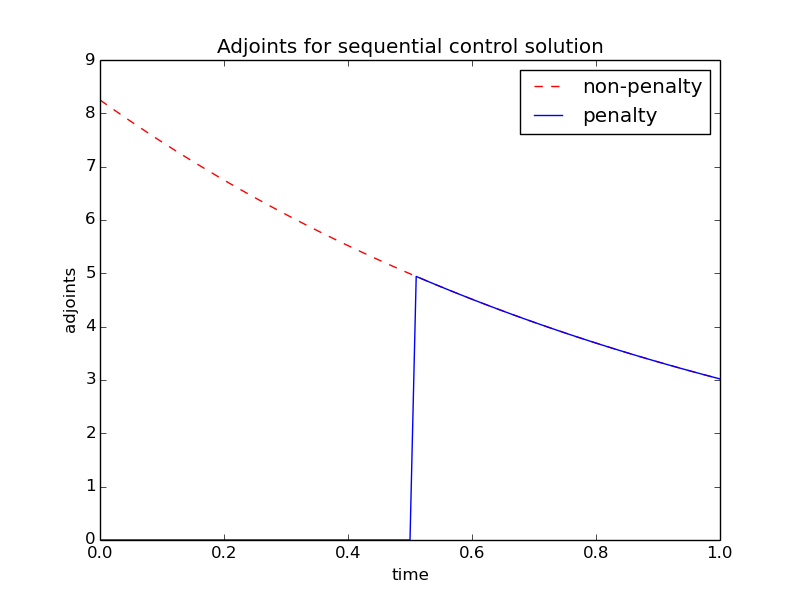
\includegraphics[width=\linewidth]{adjoint.png}
  \caption{Due to zero difference in state equation jumps, the adjoint in the penalty case has a big jump. This jump will show up in the gradient}
  \label{Fig 1}
\end{figure}
\begin{figure}
  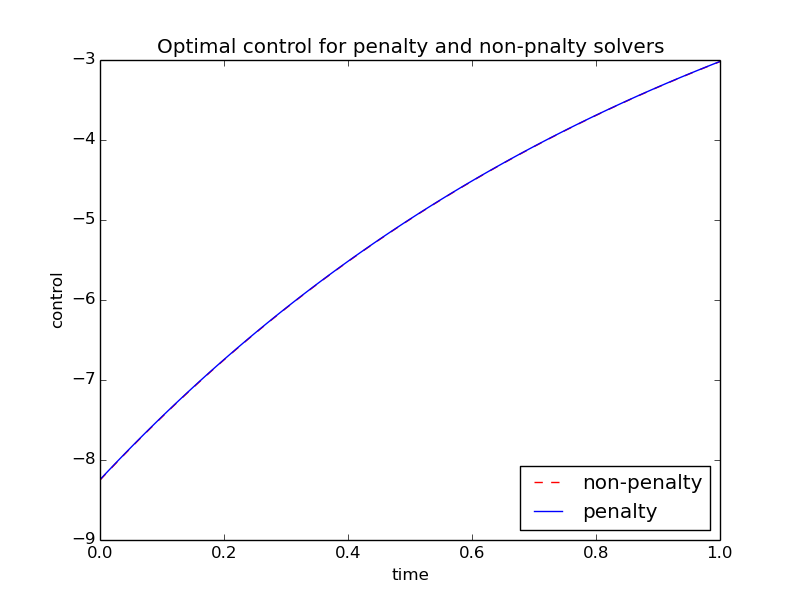
\includegraphics[width=\linewidth]{control.png}
  \caption{Results of non-penalty and penalty solver, when using $u^*$ as initial guess for penalty solver}
  \label{Fig 2}
\end{figure}

\end{document}